
\subsubsection{13.10.14}

\begin{enumerate}
	\item Время начала и окончания собрания:\newline
	21:00 - 21:30
	\item Цели собрания:\newline
	\begin{enumerate}
	  \item Установить направляющие на робота.\newline
	  
	  \item Разработать концепцию механизма для закидывания мячей в подвижные корзины.\newline
	  
    \end{enumerate}
	\item Проделанная работа:\newline
	\begin{enumerate}
	  \item Поскольку в нашу стратегию входило возить подвижную корзину за собой сзади, было решено установить на последней направляющей ось, вокруг которой мог бы вращаться ковш с мячами. Сверху ковша будет помещена трубка диаметром чуть больше диаметра большего шарика, которая будет поворачиваться вокруг оси вместе с ним и в тот момент, когда ковш будет находиться выше трубки, мячи по ней будут скатываться назад, за робота, туда, где расположена корзина.\newline
	  
	  \begin{figure}[H]
	  	\begin{minipage}[h]{0.2\linewidth}
	  		\center  
	  	\end{minipage}
	  	\begin{minipage}[h]{0.6\linewidth}
	  		\center{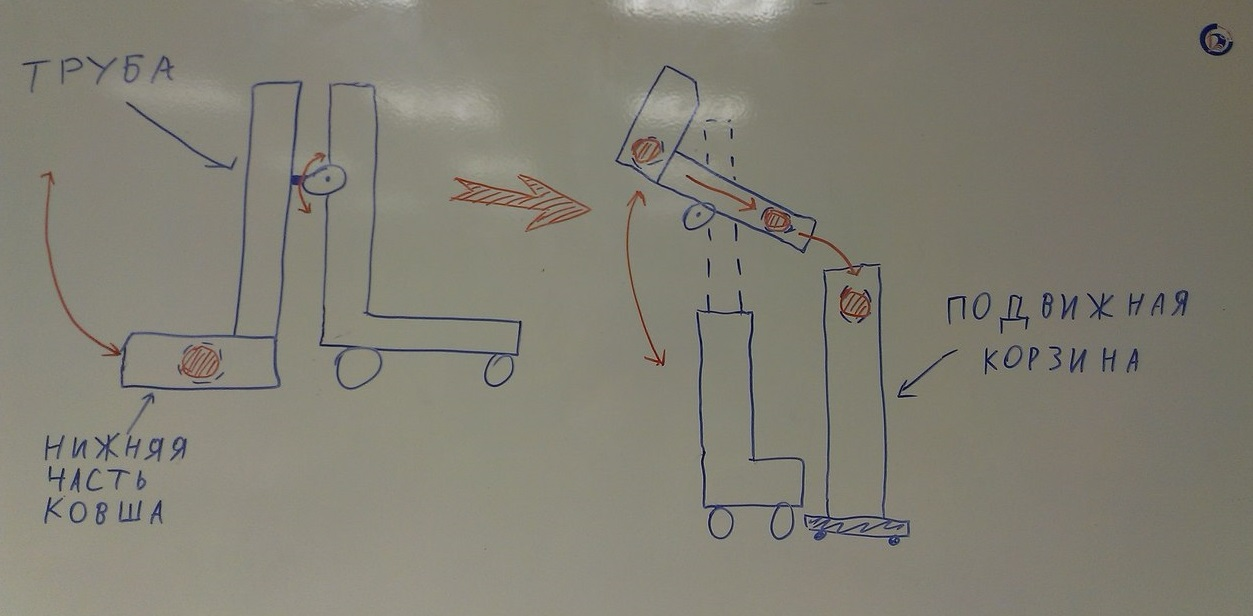
\includegraphics[height=0.9\measurepage,width=1\linewidth]{days/13.10.14/images/01}}
	  		\caption{Идея для ковша}
	  	\end{minipage}
	  \end{figure}
      
      \item  Было подсчитано, что оптимальным местом расположения оси, вокруг которой должен будет вращаться ковш, является помещение ее в 20 сантиметрах от нижнего края последнего сегмента направляющих. Дополнительный прирост высоты подъема ковша позволил отказаться от одной пары 30-сантиметровых мебельных реек. Таким образом, у нас осталось три пары мебельных реек рабочей высотой в 105 сантиметров и механизм для закидывания мячей в корзины, находящийся на стадии разработки.\newline
      
      \item  Измененные направляющие были установлены на робота.\newline
      
      \item  После установки направляющих было решено протестировать работу подъемника. Ремень хорошо справлялся с задачей, однако оси прогибались, испытывая сильные нагрузки, из чего был сделан вывод, что нам необходимы более прочные оси. Кроме того, рейки раздвигались неодинаково, поэтому было решено попарно жестко скрепить  их друг с другом. Критических проблем в системе подъемника обнаружено не было.\newline
      
      \begin{figure}[H]
      	\begin{minipage}[h]{0.47\linewidth}
      		\center{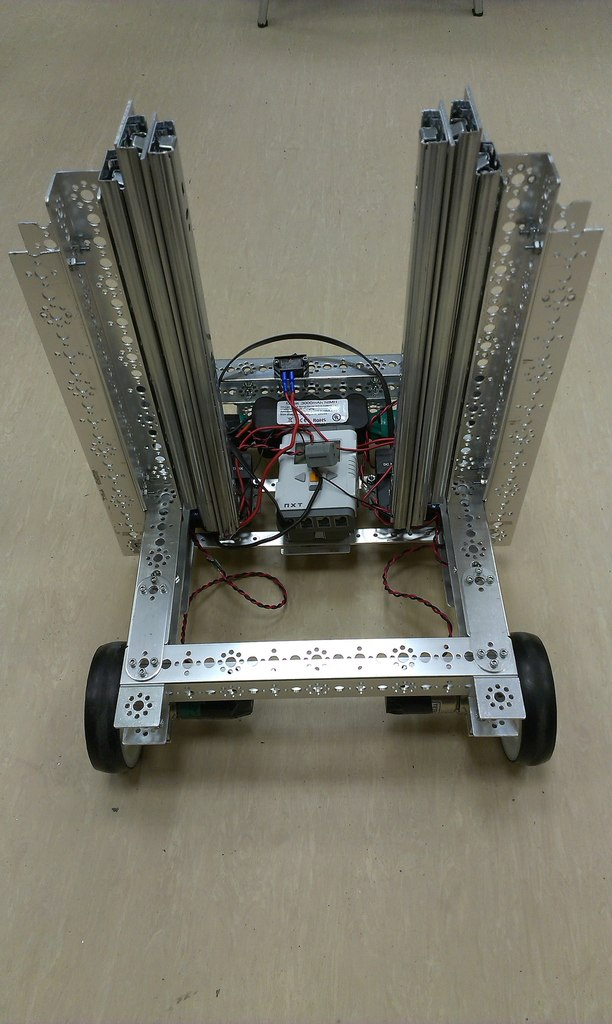
\includegraphics[height=0.95\measurepage]{days/13.10.14/images/02}}
      	\end{minipage}
      	\hfill
      	\begin{minipage}[h]{0.47\linewidth}
      		\center{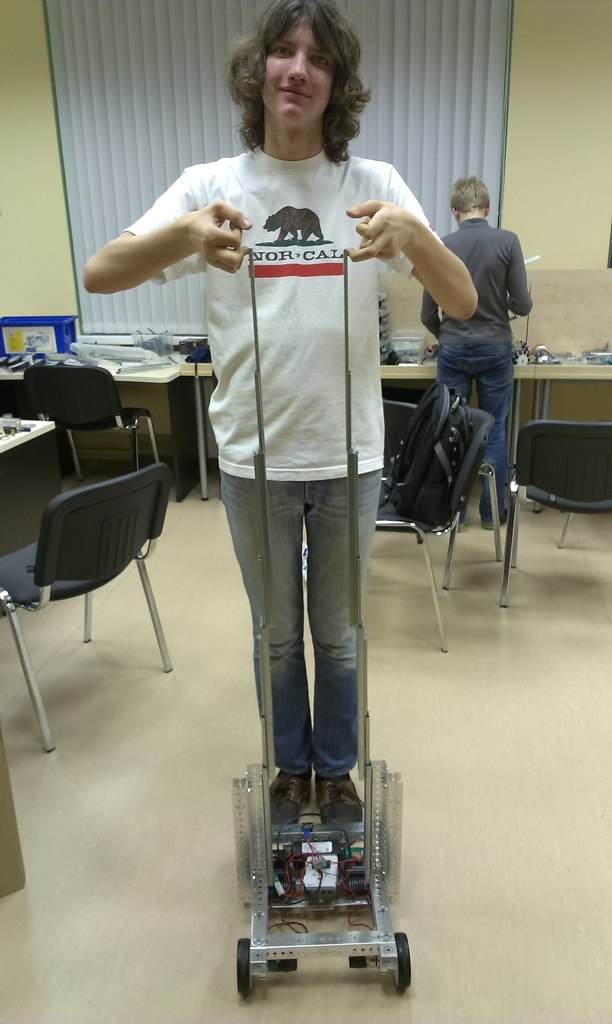
\includegraphics[height=0.95\measurepage]{days/13.10.14/images/03}}
      	\end{minipage}
      	\caption{Робот с установленными на него направляющими}
      \end{figure}
      
    \end{enumerate}
    
	\item Итоги собрания: \newline
	\begin{enumerate}
	  \item  Направляющие установлены на робота. Их конструкция упрощена.\newline
	  
      \item  Разработана концепция механизма закидывания мячей в корзины.\newline
    \end{enumerate}
    
	\item Задачи для последующих собраний:\newline
	\begin{enumerate}
	  \item Собрать устройство для вращения ковша.\newline
	  
	  \item Найти и купить более прочные оси для подъемника.\newline
	  
	  \item Купить еще один алюминиевый профиль для жесткого закрепления мебельных направляющих между собой.\newline

    \end{enumerate}     
\end{enumerate}

\fillpage
